\documentclass[12pt]{article}
\usepackage[margin = 1in]{geometry}
\usepackage{amsmath}
\usepackage{stata}
\usepackage[pdftex]{graphicx}
\usepackage{bibentry}
\usepackage{ccaption}
\usepackage{fourier}


\usepackage[colorlinks=true,
                      pdfstartview=FitV,
                      urlcolor=blue,
]{hyperref}

\usepackage{natbib}

\begin{document}

\thispagestyle{empty}%

\setlength{\parskip}{1ex plus 0.5ex minus 0.2ex}

\setcounter{secnumdepth}{-2}


\begin{flushleft}
Vanderbilt University\\Leadership, Policy and Organizations\\Class Number 9522\\ Spring 2017\\
\end{flushleft}

\begin{center}
\textbf{Regression Models for Binary Outcomes}
\end{center}


There are many times when the dependent variables  do not come in the
nice, continuous, normally distributed form that we assume in
introductory regression courses. The real world, being less generous,
provides data in all kinds of forms. The first thing to think about is
the underlying \textit{Data Generation Mechanism}. What provides the
outcome you see? If you reasonably think that the data should be a
continuous variable with a more or less normal distribution, you can
use a variety of transformations to get it where you need it to
be. However, if the underlying DGM is decidedly non-normal, you need
to look into alternative models.

A quite common occurrence in education research is a DGM that provides
binary data. A partial list includes:

\begin{itemize}
\item High School/ College Graduation: yes or no?

\item College Entry: yes or no?

\item Departure from teaching: yes or no?

\item Failure to make AYP: yes or no?

\item Employment after graduation: yes or no?


\end{itemize}

All of these share a common DGM that gives a binary response. We'll
consider two models to deal with this kind of outcome variable: the
outmoded linear probability model, and logistic regression. 


\section{Linear Probability Model}

In this class we'll consider a model which predicts the binary outcome
of college attendance as a function of ses, demographics, and test
scores. To start, we could esimtate this using good old OLS and
see what happens. This is known as a \textit{linear probability
  model}.

\begin{equation*}
  y_i=\mathbf{\beta_0 + x_i\beta} + e_i \qquad, y \in {0,1}
\end{equation*}



To do this in Stata, we would run the following:



\begin{stlog}

. /* Linear Probability Model */
. 
. reg `y' `ses' `demog' `tests'

      Source |       SS       df       MS              Number of obs =   13284
-------------+------------------------------           F(  9, 13274) =  374.14
       Model |  496.008461     9  55.1120512           Prob > F      =  0.0000
    Residual |  1955.28354 13274  .147301759           R-squared     =  0.2023
-------------+------------------------------           Adj R-squared =  0.2018
       Total |  2451.29201 13283  .184543552           Root MSE      =   .3838

------------------------------------------------------------------------------
    f2evratt |      Coef.   Std. Err.      t    P>|t|     [95% Conf. Interval]
-------------+----------------------------------------------------------------
      byses1 |   .1230284   .0051494    23.89   0.000     .1129347     .133122
       amind |  -.0799666   .0375121    -2.13   0.033    -.1534955   -.0064376
       asian |   .1061966   .0118984     8.93   0.000     .0828741    .1295192
       black |   .0664432   .0107626     6.17   0.000     .0453469    .0875395
    hispanic |   .0224763    .010479     2.14   0.032     .0019359    .0430167
 multiracial |   -.045084   .0158417    -2.85   0.004    -.0761361    -.014032
       bysex |   .0863008   .0067759    12.74   0.000     .0730191    .0995824
    bynels2m |   .0069647   .0003931    17.72   0.000     .0061943    .0077352
    bynels2r |   .0047414   .0005583     8.49   0.000      .003647    .0058357
       _cons |   .1329982   .0183363     7.25   0.000     .0970564      .16894
------------------------------------------------------------------------------
 
  \end{stlog}

We'll use this coefficients as a baseline to compare with the logistic regressions we'll run later. 


\begin{figure}[h]
  \centering
  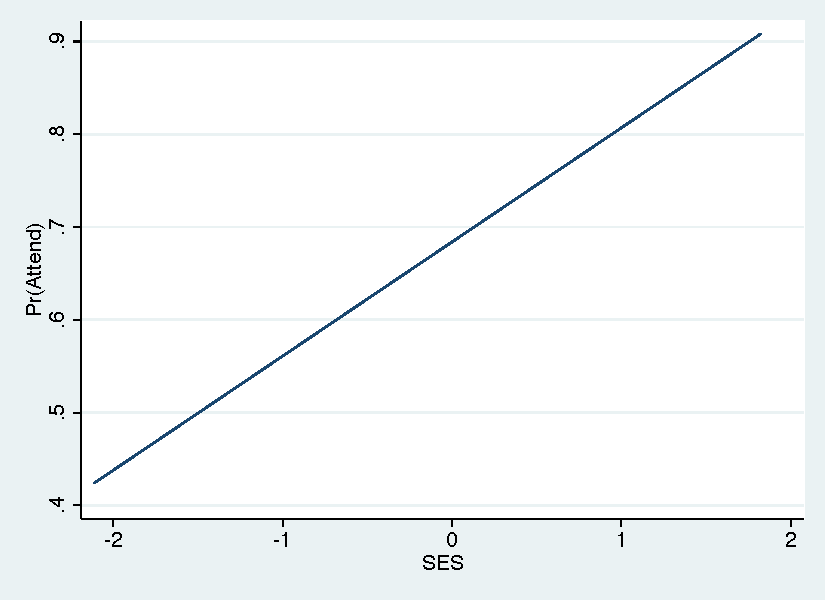
\includegraphics[width=\textwidth]{lpm}
  \caption{Predicted Probability of Attendance by SES, LPM}
\end{figure}



There are several problems with the LPM:


\subsection{Probabilities outside of 0,1}

In an ironic twist, the linear probability model does not give back
probabilities. Instead, it fits a linear model to the data and gives
predictions based on this assumption. This means that there can be
predicted probabilities outside of 0,1. Of course, you can always just
recode these predictions to be 1 or 0 but we generally try to avoid
making up data. 


\subsubsection{Quick Exercise}

Run a regression that models attendance as a function of test
scores. See if there are any predicted probabilities that are outside of the range 0,1. 


\subsection{Non-Normality of Errors}

The results from the LPM produce residuals that are far from normal,
they are in fact binomial. This follows from

\begin{equation*}
  y_i=1 \Rightarrow e_i=1-(\beta_0 + \mathbf{x_i\beta})
\end{equation*}


\begin{equation*}
  y_i=0 \Rightarrow e_i=-(\beta_0 + \mathbf{x_i\beta})
\end{equation*}

\subsubsection{Quick Exercise}

Generate the residuals from the above regression and plot them against
math test scores. 

\subsection{Heteroscedasticity}

Since the residuals are a function of $y$, this means that the residuals
are also a function of the systematic component of $y$ represented by
$x$. The variance of a binary variable is $p(1-p)$, so the variance of
$e$ is:

\begin{equation}
  V(e)=(\beta_0 + \mathbf{x_i\beta})[1-((\beta_0 + \mathbf{x_i\beta}))]
\end{equation}

When residuals are dependent on the data, we have heteroscedasticity. 


\subsubsection{Quick Exercise}

Plot the residuals against the test scores variable. What do you see? 

Of course, all of the normal methods for dealing with
heteroscedasticity work here. Instead of the above, we can run
ordinary least squares with robust standard errors, which will deal
with the non-iid terms adequately. 

\begin{stlog}

. reg `y' `ses' `demog' `tests', robust

Linear regression                                      Number of obs =   13284
                                                       F(  9, 13274) =  408.19
                                                       Prob > F      =  0.0000
                                                       R-squared     =  0.2023
                                                       Root MSE      =   .3838

------------------------------------------------------------------------------
             |               Robust
    f2evratt |      Coef.   Std. Err.      t    P>|t|     [95% Conf. Interval]
-------------+----------------------------------------------------------------
      byses1 |   .1230284   .0051319    23.97   0.000     .1129691    .1330876
       amind |  -.0799666   .0453305    -1.76   0.078    -.1688208    .0088877
       asian |   .1061966   .0105472    10.07   0.000     .0855226    .1268707
       black |   .0664432   .0117838     5.64   0.000     .0433454    .0895411
    hispanic |   .0224763     .01161     1.94   0.053     -.000281    .0452335
 multiracial |   -.045084   .0166198    -2.71   0.007    -.0776612   -.0125069
       bysex |   .0863008   .0067757    12.74   0.000     .0730194    .0995821
    bynels2m |   .0069647   .0004003    17.40   0.000       .00618    .0077495
    bynels2r |   .0047414    .000568     8.35   0.000      .003628    .0058547
       _cons |   .1329982   .0195842     6.79   0.000     .0946104    .1713861
------------------------------------------------------------------------------

. 
\end{stlog}

\section{Logit Model}

Given the above theoretical problems with the LPM, almost all analysts
favor the use of models specifically for binary variables.

\subsection{Generalized Linear Models}

A \textit{Generalized Linear Model} posits that $y$ is a function of
the independent variables and the coefficients or other parameters via
a \textit{link function}:

\begin{equation*}
  P(y|\mathbf{x})=G(\beta_0 + \mathbf{x_i\beta})
\end{equation*}

In our case, we're interested in the probability that $y$ is 1

\begin{equation*}
  P(y=1|\mathbf{x})=G(\beta_0 + \mathbf{x_i\beta})
\end{equation*}

There are several functions that ``map'' onto a 0,1 continuum. The
most commonly used is the logistic function, which gives us the
\textit{logit model}.

The logistic function is given by:

\begin{equation*}
  f(x)=\frac{1}{1+exp^{-k(x-x_0)}}
\end{equation*}

Mapped onto our GLM, this gives us: 

\begin{equation*}
  P(y=1|\mathbf{x})=\frac{exp(\beta_0 + \mathbf{x_i\beta})}{1+exp(\beta_0 + \mathbf{x_i\beta})}
\end{equation*}

The critical thing to note about the above is that the link function
maps the entire result of estimation $(\beta_0 + \mathbf{x_i\beta})$
onto the 0,1 continuum. Thus, the change in the $P(y=1|\mathbf{x})$ is
a function of all of the independent variables and coefficients
together, \textit{not} one at a time. 

What does this mean? It means that the coefficients can only be
interpreted on the \textit{logit} scale, and don't have the normal
interpretation we would use for OLS regression. Instead, to understand
what the logistic regression coefficients mean, you're going to have
to convert the entire term $(\beta_0 + \mathbf{x_i\beta})$ to the
probability scale, using the inverse of the function. 

\subsection{Maximum Likelihood Estimation}

The other important thing to know about the logit model is that it is
estimated via maximum likelihood. This is in contrast to OLS, which we
estimate via direct computation. You could, given the time and the
willingness, sit down and compute the estimates for an OLS model. For
a MLE model, we use a likelihood function which gives us the
likelihood of the data given a certain set of parameters. The computer then
adjusts the estimates of the parameters, checks to see if the
likelihood has gone up or down, and repeats. The algorithm keeps on
looking for the parameters that make the data most likely. This stops
at a pre-set point when improvements in the likelihood are small. this
condition is called \textit{convergence}

To run a logistic regression in Stata, enter:

\begin{stlog}
  
. /*Logistic Regression */
. 
. logit `y' `ses' `demog' `tests'

Iteration 0:   log likelihood = -7383.1405  
Iteration 1:   log likelihood = -5998.4224  
Iteration 2:   log likelihood = -5882.6198  
Iteration 3:   log likelihood = -5881.8938  
Iteration 4:   log likelihood = -5881.8937  

Logistic regression                               Number of obs   =      13284
                                                  LR chi2(9)      =    3002.49
                                                  Prob > chi2     =     0.0000
Log likelihood = -5881.8937                       Pseudo R2       =     0.2033

------------------------------------------------------------------------------
    f2evratt |      Coef.   Std. Err.      z    P>|z|     [95% Conf. Interval]
-------------+----------------------------------------------------------------
      byses1 |   .9044976   .0375964    24.06   0.000     .8308101    .9781852
       amind |  -.2907766   .2208319    -1.32   0.188    -.7235993     .142046
       asian |   1.024893   .0997533    10.27   0.000     .8293798    1.220406
       black |   .4880564   .0687739     7.10   0.000      .353262    .6228508
    hispanic |   .3010218   .0673856     4.47   0.000     .1689485    .4330951
 multiracial |  -.2907231   .1021569    -2.85   0.004    -.4909469   -.0904993
       bysex |   .5852038   .0470378    12.44   0.000     .4930114    .6773962
    bynels2m |   .0461185    .002718    16.97   0.000     .0407913    .0514457
    bynels2r |   .0308627   .0037971     8.13   0.000     .0234205    .0383049
       _cons |  -2.684406    .124637   -21.54   0.000     -2.92869   -2.440122
------------------------------------------------------------------------------

. 
. est store full_model

. 
. gen mysample=e(sample)

\end{stlog}

The iterations refer to the steps as Stata computes the log likelihood
and then checks for convergence. You then get the final log
likelihood, the number of observations, the $\chi^2$ statistics for
the likelihood ratio test, the p value for that $\chi^2$ and the
Pseudo $R^2$. The coefficient table should look generally familiar. 


\subsection{Interpretation of Results}

The coefficients from a logit model are not directly interpretable in
the same way as OLS estimates. This is because they are linear only in
the log odds, which is not a way that (ordinary) humans think about
the world. We are interested in the changes in the $P(y=1)$, which
means that we have to take into account the \textit{whole} model,
since this is what is mapped onto the (0,1) scale. 


\subsubsection{Quick Exercise}

Run a logistic regression predicting  college attendance by
math scores. Generate a predicted outcome, and plot this against
math scores. Use the form \texttt{predict yhat, pr} to get predicted
probabilities for $y=1$. 


\subsection{Generating Probabilities}

Since we are primarily interested in the probability that $y=1$, the
best course to take to interpret coefficients is to demonstrate what
happens to the dependent variable as we allow certain independent
variables to move across their range. In Stata, the \texttt{margins}
is indispensable for this task.

Reporting these results well takes some time and some effort. The
analyst needs to think carefully about the likely changes in the
independent variables, and the right levels at which to hold the other
variables constant. For our first take, let's let race vary and then
generate margins for a series of values of SES: 

\begin{stlog}

. /* Generate predicted probabilites over range of ses*/
. 
. local x byses1

. 
. sum `x', detail

            socio-economic status composite, v.1
-------------------------------------------------------------
      Percentiles      Smallest
 1%        -1.54          -2.11
 5%        -1.18          -2.11
10%         -.95          -1.97       Obs               15325
25%          -.5          -1.97       Sum of Wgt.       15325

50%          .04                      Mean           .0426499
                        Largest       Std. Dev.      .7429194
75%          .59            1.8
90%         1.05            1.8       Variance       .5519293
95%         1.26           1.81       Skewness      -.0235649
99%         1.55           1.82       Kurtosis       2.354114

. 
. local no_steps=20

. 
. local mymin=r(min)

. local mymax=r(max)

. local diff=`mymax'-`mymin'

. local step=`diff'/`no_steps'

. 
.     
. margins , predict(xb) ///
>     at((mean) _continuous ///
>         (min) `demog' ///
>         `x'=(`mymin'(`step')`mymax') ///          
>        ) ///
>       post

Adjusted predictions                              Number of obs   =      13284
Model VCE    : Robust

Expression   : Linear prediction, predict(xb)

1._at        : byses1          =       -2.11
               amind           =           0 (min)
               asian           =           0 (min)
               black           =           0 (min)
               hispanic        =           0 (min)
               multiracial     =           0 (min)
               bysex           =           1 (min)
               bynels2m        =     46.1288 (mean)
               bynels2r        =    30.23475 (mean)
\end{stlog}

We can plot the results from this margins command like so: 



\begin{figure}[h]
  \centering
  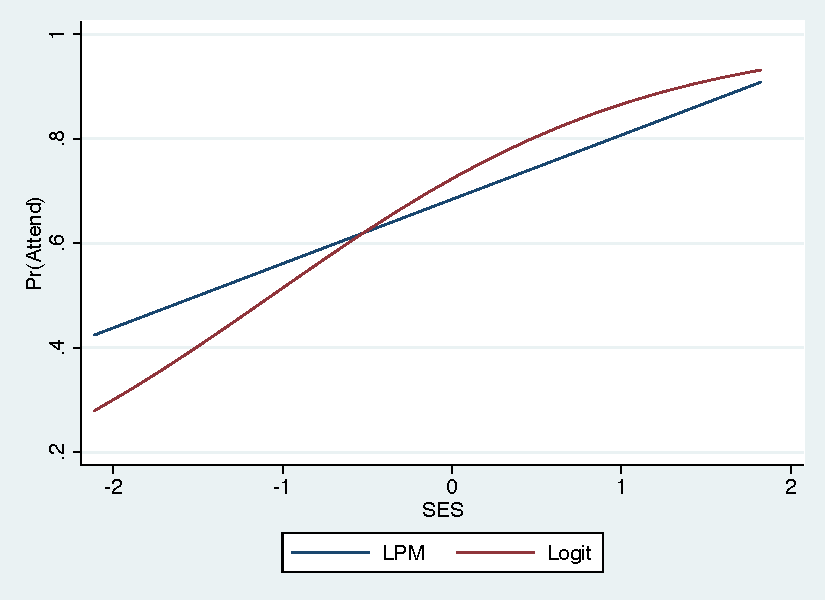
\includegraphics[width=\textwidth]{logit_basic}
  \caption{Predicted Probability of Attendance by SES, Logit and LPM}
\end{figure}


For another example, we'll let ses and race vary, holding other
variables constant. The resulting graphic shows the predicted change
in the probability of college attendance as these two variables
change. 


\begin{figure}[h]
  \centering
  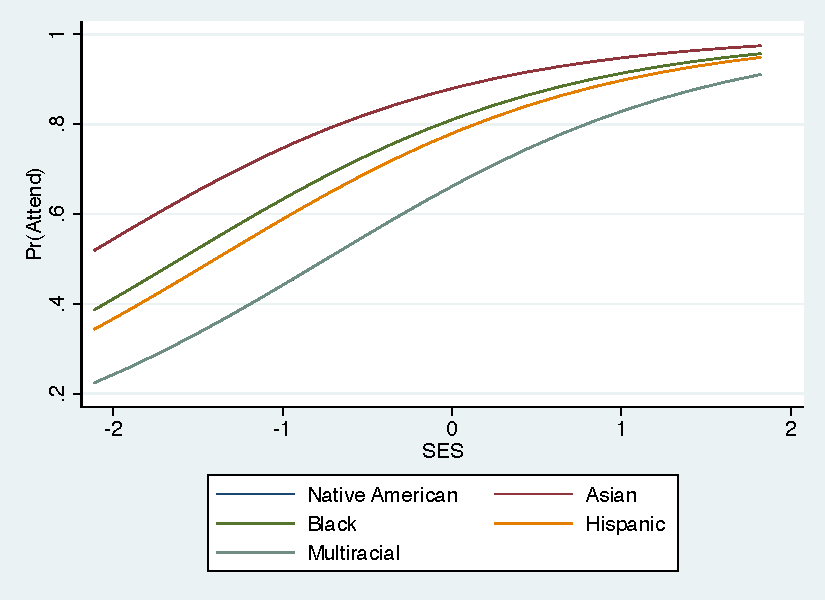
\includegraphics[width=\textwidth]{logit_race}
  \caption{Predicted Probability of Attendance by SES}
\end{figure}


\subsubsection{Quick Exercise}

Generate a set of predicted probabilities from our model that show the
predicted change in probability of college attendance for white women
with high, medium and low test scores, holding
other variables constant at a reasonable level. Do this
for the entire range of ses and plot the result. 




\subsection{Generating Marginal Effects}

The marginal effect of a covariate is the predicted change in the
probability of the outcome as a result of a one unit change in the
covariates, with all other covariates held constant at some level. For
logistic regression, it's most common to hold all other variables at
their means, but it's not the only way to go. 

In Stata, marginal effects can be computed quickly using the
\texttt{margins} command. Running this for all variables with the
\texttt{dydx} option will give you the marginal effect of each
covariate, interpreted as a change in probability of the outcome for a
one unit change in the indepndent variable, holding all other
variables constant. 


\begin{stlog}
. /* Generating marginal effects */
. margins, dydx(*) /*for all coefficients, default is to hold others at mean */  

Average marginal effects                          Number of obs   =      13284
Model VCE    : OIM

Expression   : Pr(f2evratt), predict()
dy/dx w.r.t. : byses1 amind asian black hispanic multiracial bysex bynels2m bynels2r

------------------------------------------------------------------------------
             |            Delta-method
             |      dy/dx   Std. Err.      z    P>|z|     [95% Conf. Interval]
-------------+----------------------------------------------------------------
      byses1 |   .1295129   .0050031    25.89   0.000     .1197071    .1393188
       amind |  -.0416356   .0316113    -1.32   0.188    -.1035926    .0203213
       asian |    .146752   .0141156    10.40   0.000     .1190861     .174418
       black |   .0698837   .0097859     7.14   0.000     .0507036    .0890637
    hispanic |   .0431026   .0096314     4.48   0.000     .0242253    .0619799
 multiracial |   -.041628   .0146135    -2.85   0.004      -.07027    -.012986
       bysex |    .083794    .006603    12.69   0.000     .0708524    .0967355
    bynels2m |   .0066036    .000375    17.61   0.000     .0058685    .0073387
    bynels2r |   .0044192   .0005392     8.20   0.000     .0033623     .005476
------------------------------------------------------------------------------

. 
\end{stlog}

 A notable
exception to analysts preferring a nonlinear model for a binary
dependent variable would be Angrist and Pischke, who say ``The upshot of this
discussion is that while a nonlinear model may fit the CEF
(cnoditional expectation function) for LDVS (lmitied dependent
variables) more closely than a linear model, when it comes to marginal
effects, this probably matters little. This optimistic conclusion is
not a theorem, but . .  it seems to be fairly robustly true.''

\subsection{Reporting Odds Ratios}

The odds ratio for any coefficient is the predicted change in odds for
a one unit change in the covariate, while holding all other variables
constant (usually at their mean). The simplest way to obtain odds
ratios from Stata is to run the logit model with the \texttt{logistic}
command:


To get the odds ratios, we calculate the exponent of the
coefficients. The result show the ratio of the probability that $y=1$
when we shift the covariate of interest by a specific amount. In
Stata, the default is one unit, but this can be adjusted. The
interpretation of this is that after a change of the specified size
the odds are so much larger or smaller. 

\begin{stlog}
  . 
. 
. listcoef /*Display odds ratios from model in memory */

logit (N=13284): Factor Change in Odds 

  Odds of: Yes vs No

----------------------------------------------------------------------
    f2evratt |      b         z     P>|z|    e^b    e^bStdX      SDofX
-------------+--------------------------------------------------------
      byses1 |   0.90450   24.058   0.000   2.4707   1.9612     0.7447
       amind |  -0.29078   -1.317   0.188   0.7477   0.9743     0.0894
       asian |   1.02489   10.274   0.000   2.7868   1.3480     0.2913
       black |   0.48806    7.097   0.000   1.6291   1.1790     0.3373
    hispanic |   0.30102    4.467   0.000   1.3512   1.1098     0.3462
 multiracial |  -0.29072   -2.846   0.004   0.7477   0.9397     0.2138
       bysex |   0.58520   12.441   0.000   1.7954   1.3396     0.4997
    bynels2m |   0.04612   16.968   0.000   1.0472   1.8722    13.5976
    bynels2r |   0.03086    8.128   0.000   1.0313   1.3370     9.4115
----------------------------------------------------------------------

\end{stlog}

Odds ratios for negative coefficients can be hard to interpret, so you
can also ask Stata to reverse the interpretation, like so: 

\begin{stlog}
  
.
. listcoef, reverse /* Reveres interpretation, helps with negative coefs */

logit (N=13284): Factor Change in Odds 

  Odds of: No vs Yes

----------------------------------------------------------------------
    f2evratt |      b         z     P>|z|    e^b    e^bStdX      SDofX
-------------+--------------------------------------------------------
      byses1 |   0.90450   24.058   0.000   0.4047   0.5099     0.7447
       amind |  -0.29078   -1.317   0.188   1.3375   1.0263     0.0894
       asian |   1.02489   10.274   0.000   0.3588   0.7419     0.2913
       black |   0.48806    7.097   0.000   0.6138   0.8482     0.3373
    hispanic |   0.30102    4.467   0.000   0.7401   0.9010     0.3462
 multiracial |  -0.29072   -2.846   0.004   1.3374   1.0641     0.2138
       bysex |   0.58520   12.441   0.000   0.5570   0.7465     0.4997
    bynels2m |   0.04612   16.968   0.000   0.9549   0.5341    13.5976
    bynels2r |   0.03086    8.128   0.000   0.9696   0.7479     9.4115
----------------------------------------------------------------------

\end{stlog}


Odds ratios seem simple but are not really--they are a specific way of
calculating predicted probabilities that many times allow the analyst
to avoid thinking carefully about the results. Use them with care. Or
not at all. Really, you shouldn't use them. Nobody does a good job
writing them up. 


\subsubsection{Quick Exercise}

Interpret the odds ratio for income from the above regression. Write
down your answer. Get the marginal effects for all of the variables, but this time hold all of
the other variables constant at their medians. 


\subsection{Hypothesis Testing}

To test whether an individual coefficient is 0, we use  a similar
method as in OLS, except the distribution of the test statistic is the
Normal distribution not the T distribution. For that reason, we report
z and not t statistics. 


\subsection{Likelihood Ratio Test}

To test whether a subset of coefficients jointly increase model fit,
we use the likelihood ratio test. This is two times the difference in
log likelihoods, and can be done quite easily in Stata. To test the
full model in our example against one with just the kids variables, we
would run:


In Stata, the test is: 

\begin{stlog}


. 
. lrtest full_model ses

Likelihood-ratio test                                 LR chi2(8)  =   1398.05
(Assumption: ses nested in full_model)                Prob > chi2 =    0.0000

. 
. quietly logit `y'  `demog' if mysample==1

. 
. est store demog

. 
. lrtest full_model demog

Likelihood-ratio test                                 LR chi2(3)  =   2542.87
(Assumption: demog nested in full_model)              Prob > chi2 =    0.0000

. 
. quietly logit `y' `tests' if mysample==1

. 
. est store tests

. 
. lrtest full_model tests

Likelihood-ratio test                                 LR chi2(7)  =    860.54
(Assumption: tests nested in full_model)              Prob > chi2 =    0.0000


\end{stlog}



\subsection{Goodness of Fit}

Goodness of fit in this context is somewhat more complex than in
OLS. There are three basic methods: the Chi Square Test, McFadden's
Pseudo $R^2$, and the percent correctly predicted method.

\subsection{Chi Square Test}

The Chi Square Test, like the F test, tests the null hypothesis that
all of the coefficients are 0. Like the F test, it is  a very weak
test. 

\subsection{Pseudo $R^2$}

The pseudo $R^2$ is just like it sounds--not a real $R^2$. It shares
the same general interpretation of $R^2$--levels close to 0 are bad,
levels close to one are good. 

\subsection{Percent Correctly Predicted}

The last method to use is to think about the percent correctly
predicted. This is fairly intuitive and easy to do. However, the key
concept here is the threshold of correctness. Generally, we use .5
probability as the threshold, but there's nothing magic about
.5. Depending on the application, we might be more comfortable with a
lower false negative, or a lower false positive---it just depends. 

The command in Stata is:


\begin{stlog}

. /* Percent Correctly Predicted  */
. 
. estat classification

Logistic model for f2evratt

              -------- True --------
Classified |         D            ~D  |      Total
-----------+--------------------------+-----------
     +     |      9322          2068  |      11390
     -     |       719          1175  |       1894
-----------+--------------------------+-----------
   Total   |     10041          3243  |      13284

Classified + if predicted Pr(D) >= .5
True D defined as f2evratt != 0
--------------------------------------------------
Sensitivity                     Pr( +| D)   92.84%
Specificity                     Pr( -|~D)   36.23%
Positive predictive value       Pr( D| +)   81.84%
Negative predictive value       Pr(~D| -)   62.04%
--------------------------------------------------
False + rate for true ~D        Pr( +|~D)   63.77%
False - rate for true D         Pr( -| D)    7.16%
False + rate for classified +   Pr(~D| +)   18.16%
False - rate for classified -   Pr( D| -)   37.96%
--------------------------------------------------
Correctly classified                        79.02%
--------------------------------------------------


\end{stlog}

The resulting table (also known as a confusion matrix) gives you both
sensitivity (the proportion of 1's that are correctly identified) and
specificity (the proportion of 0's correctly identified). Depending on
the application, one or the other may be more important to the
analyst.


ROC (an acronym for receiver-operator characteristic) goes some way
towards overcoming the problem of choosing a threshold. The ROC
considers what happens to the classification rate as the
classification threshold ranges from zero to one.  The ROC is based on
changing the classification threshold. When doing this, the number of
``true positive'' classifications changes in inverse proportion to the
number of ``false positive'' classifications. ROC analysis is usually
done graphically, plotting the TPF (true positive fraction, TPF = 1 -
FNF), versus the FPF (false positive fraction) as the classification
threshold varies. The resulting function is defined on the unit
square, and the area under the ROC curve c is interpreted as a measure
of the classification success of the model. A value of c = .5
indicates random predictions and a value of c = 1 indicates perfect
prediction.

The command in Stata is:

\begin{stlog}

. /*Area under Receiver/Operator Characteristic Curve */
. 
. lroc 

Logistic model for f2evratt

number of observations =    13284
area under ROC curve   =   0.8013

\end{stlog}

You can also compare models and do a graphical comparison, like so: 

\begin{stlog}

.   est restore ses
(results ses are active now)

. 
. predict xb_ses, xb
(964 missing values generated)

. 
. est restore full_model
(results full_model are active now)

. 
. predict xb_full, xb
(964 missing values generated)

.  
. roccomp f2evratt xb_full xb_ses, graph summary

                              ROC                    -Asymptotic Normal--
                   Obs       Area     Std. Err.      [95% Conf. Interval]
-------------------------------------------------------------------------
xb_full          13284     0.8013       0.0043        0.79293     0.80960
xb_ses           13284     0.7300       0.0048        0.72056     0.73934
-------------------------------------------------------------------------
Ho: area(xb_full) = area(xb_ses)
    chi2(1) =   345.06       Prob>chi2 =   0.0000

\end{stlog}


\begin{figure}
  \centering
  \caption{Area Under ROC Curve: Comparing Two Models}
 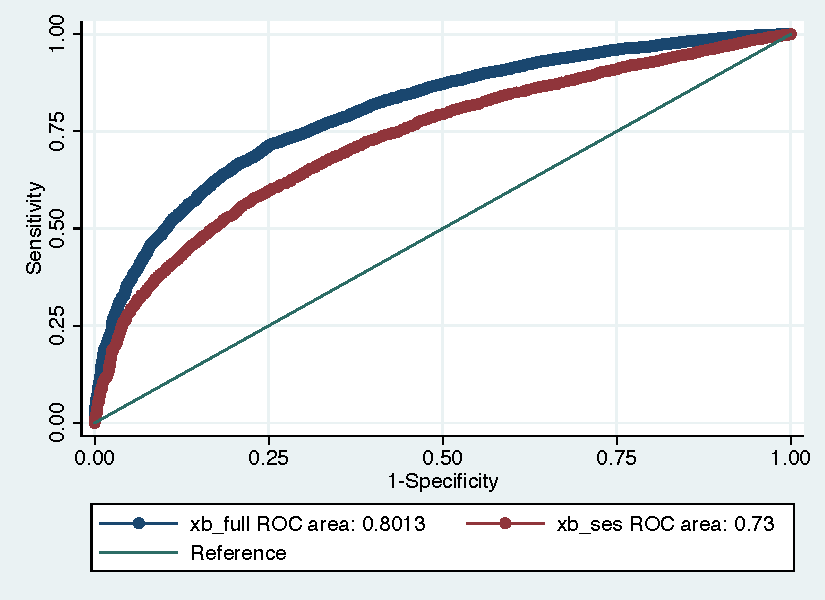
\includegraphics{roc_curve}
  \label{fig:roccurve}
\end{figure}


\end{document}
